\examsetup{February 24, 2016}{Spring 2016}
\vspace*{1.15in}
\begin{center}
{\sffamily\bfseries\Large Texas A\&M University\\
Department of Electrical and Computer Engineering\par}
\vspace{.35in}
{\sffamily\bfseries\large ECEN 474/704 -- (Analog) VLSI Circuit Design\par}
\vspace{.35in}
{\sffamily\bfseries\large Spring 2016\par}
\vspace{.28in}
{\sffamily\bfseries\large Exam \#1\par}
\vspace{.28in}
{\sffamily\bfseries\large Instructor: Sam Palermo\par}
\end{center}
\vspace{.35in}
\begin{itemize}[leftmargin=24pt,itemsep=1pt,topsep=0pt]
\item Please write your name in the space provided below
\item Please verify that there are \textbf{5 pages} in your exam
\item You may use \underline{one} double-sided page of notes and equations for the exam
\item Good Luck!
\end{itemize}
\vspace{.65in}
\begin{tabular}{|c|c|c|}\hline
Problem & Score & Max Score\\\hline
1&&40\\\hline
2&&40\\\hline
3&&20\\\hline
\textbf{Total}&&\textbf{100}\\\hline
\end{tabular}
\vfill
Name: \hrulefill\par
\vspace{8pt}
UIN: \hrulefill
\newpage

\begingroup
\fontsize{10.8}{12.2}\selectfont
\setlength{\parskip}{4pt}
\textbf{Problem 1 (40 points)}\par
\textbf{For the layout below, assume that all the commonly labeled diffusion areas are connected with the appropriate metal layers. Assume that $V_X=1.2\,\mathrm V$, $V_Y=0\,\mathrm V$, $V_Z=0.4\,\mathrm V$, $V_{T0}=0.7\,\mathrm V$, $\gamma=0$, and that all Spice parameters are given (i.e. $C_j$, $C_{jsw}$, $C_{jc}$, $C_{ox}$, $C_{ov}$). The dimensions are given in $\mu\mathrm m$, with all the poly gates having a length of $2\,\mu\mathrm m$ and $L_D=0.1\,\mu\mathrm m$.}
\begin{enumerate}[label=\alph*),leftmargin=19pt,itemsep=1pt,topsep=2pt]
\item Draw the equivalent circuit. Combine all parallel transistors and give the total width and length of the equivalent transistors. \hfill (15 points)
\item What region(s) are the transistors operating in? \hfill (5 points)
\item For node \textbf{X only}, give an expression and calculate the total gate cap. \hfill (10 points)
\item For node \textbf{Z only}, give an expression and calculate the total junction cap. Note for the perimeter terms, include the sides underneath the gate. \hfill (10 points)
\end{enumerate}

\begin{center}
\begin{minipage}[c]{.49\linewidth}\centering
\begin{tikzpicture}[x=.077cm,y=.077cm,font=\scriptsize]
\draw(-7,-7)rectangle(58,28);
\fill[gray!75](0,24)rectangle(2,26);\node[anchor=west]at(3,25){Poly};
\fill[black](22,24)rectangle(24,26);\node[anchor=west]at(25,25){Contact};
\fill[pattern=crosshatch](0,20)rectangle(2,22);\node[anchor=west]at(3,21){N+};
\fill[gray!25](22,20)rectangle(24,22);\node[anchor=west]at(25,21){M1};
\node[anchor=west]at(-4,15){P-sub};
\fill[pattern=crosshatch,pattern color=gray] (0,0)rectangle(54,10);
\draw(0,0)rectangle(54,10);
\foreach \i/\lab in {0/Y,1/Z,2/Y,3/X,4/Y,5/Z,6/Y}{
 \pgfmathsetmacro{\xx}{8*\i}
 \fill[gray!15](\xx+.6,.6)rectangle(\xx+5.4,9.4);
 \fill[black](\xx+2.1,2)rectangle(\xx+3.9,3.8);
 \fill[black](\xx+2.1,6.2)rectangle(\xx+3.9,8);
 \node[fill=white,inner sep=.2pt]at(\xx+3,5){\textbf{\lab}};
 \node at(\xx+3,-2.7){6};
}
\foreach \x in {6,14,22,30,38,46}{\fill[gray!75](\x,-1)rectangle(\x+2,13);}
\fill[gray!75](6,12)rectangle(48,14);
\fill[gray!15](25,0.5)rectangle(29,14.5);
\fill[black](26,12)rectangle(28,14);
\fill[black](26.1,2)rectangle(27.9,3.8);
\fill[black](26.1,6.2)rectangle(27.9,8);
\node[fill=white,inner sep=.2pt]at(27,5){\textbf{X}};
\draw[<->](-2,0)--node[left]{10}(-2,10);
\draw[<->](6,-4.5)--node[below]{2}(8,-4.5);
\end{tikzpicture}
\end{minipage}\hfill
\begin{minipage}[c]{.49\linewidth}\centering
\begin{circuitikz}[american,scale=.8,transform shape]
\node[nmos](m1)at(0,0){};
\node[nmos](m2)at(3,0){};
\draw(m1.S)--(0,-1)node[ground]{}--(3,-1)--(m2.S);
\draw(m1.D)--(0,1.2)node[circ]{}node[above]{$X=1.2\,\mathrm V$};
\draw(m1.G)--(-1,0)--(-1,.9)--(0,.9);
\draw(-1,.9)--(2,.9)--(2,0)--(m2.G);
\draw(m2.D)--(3,1.2)node[circ]{}node[above]{$Z=0.4\,\mathrm V$};
\node at(1.5,-1.05){$Y=0$};
\node[below]at(0,-1.5){$M_1:\ \dfrac{20}{2}$};
\node[below]at(3,-1.5){$M_2:\ \dfrac{40}{2}$};
\end{circuitikz}
\end{minipage}
\end{center}
\textbf{a.} The six unit transistors each have $W/L=10/2$. Two are connected from $X$ to $Y$ and four from $Z$ to $Y$; all gates connect to $X$. Combining them gives the two-transistor circuit above.

\textbf{b.}\quad
$M_1:\ V_{GS}=V_{DS}=1.2\,\mathrm V>V_T$, and $V_{DS}>V_{GS}-V_T$:
\boxed{\text{saturation}}.\par
\hspace*{19pt}$M_2:\ V_{GS}=1.2\,\mathrm V$, $V_{DS}=0.4\,\mathrm V<1.2-0.7=0.5\,\mathrm V$:
\boxed{\text{triode}}.

\textbf{c.} With $L_{\mathrm{eff}}=2-2(0.1)=1.8\,\mu\mathrm m$, $M_1$'s gate--drain capacitance is shorted out because gate and drain both connect to $X$. Thus
\begin{align*}
C_{gX,1}&=C_{gs,1}=\frac23(20\,\mu\mathrm m)(1.8\,\mu\mathrm m)C_{ox}
 +(20\,\mu\mathrm m)C_{ov},\\
C_{gX,2}&=C_{gs,2}+C_{gd,2}
=2\left[\frac12(40\,\mu\mathrm m)(1.8\,\mu\mathrm m)C_{ox}
 +(40\,\mu\mathrm m)C_{ov}\right].
\end{align*}
\[
\boxed{C_{gX}=96\,\mu\mathrm m^2 C_{ox}+100\,\mu\mathrm m C_{ov}.}
\]
\textbf{d.} The two $Z$ diffusion regions have total area $A_Z=2(6)(10)=120\,\mu\mathrm m^2$ and perimeter $P_Z=2\cdot2(6+10)=64\,\mu\mathrm m$, counting the gate-adjacent sides. Following the supplied solution's capacitance notation,
\begin{align*}
C_{jZ}&=A_ZC_j'+P_ZC_{jsw}'+C_{jc}\frac{W_2L_{\mathrm{eff}}}{2}\\
&=2(6)(10)\,\mu\mathrm m^2C_j'+2\cdot2(6+10)\,\mu\mathrm m C_{jsw}'
 +\frac{(40)(1.8)}2\,\mu\mathrm m^2C_{jc},\\[-4pt]
\boxed{C_{jZ}}&\boxed{=120\,\mu\mathrm m^2C_j'+64\,\mu\mathrm m C_{jsw}'+36\,\mu\mathrm m^2C_{jc}.}
\end{align*}
\endgroup
\newpage

\begingroup
\fontsize{10.8}{12.1}\selectfont
\setlength{\parskip}{5pt}
\textbf{Problem 2 (40 points)}\par
\textbf{For the transistor below, assume $V_{T0}=0.7\,\mathrm V$, $\gamma=0.45\,\mathrm V^{1/2}$, and $2\Phi_F=0.9\,\mathrm V$.}
\begin{center}
\begin{tabular}{@{}m{.23\linewidth}@{\hspace{.02\linewidth}}m{.74\linewidth}@{}}
\centering\resizebox{\linewidth}{!}{%
\begin{tikzpicture}[x=1cm,y=1cm,font=\small]
\draw[thick](.2,-.38)--(.2,.38);
\draw[thick](.34,-.32)--(.34,.32);
\draw(.34,.28)--(.65,.28)--(.65,1.05)node[circ]{}node[above]{$0.5\,\mathrm V$};
\draw(.34,-.28)--(.65,-.28)--(.65,-1)node[ground]{};
\draw(-.8,0)node[circ]{}node[left]{$0.65\,\mathrm V$}--(.2,0);
\draw(.34,0)--(1.35,0)node[circ]{}node[right]{$0.4\,\mathrm V$};
\draw[-Latex](.7,0)--(.4,0);
\node[anchor=east]at(.2,-.65){$\dfrac{10\,\mu\mathrm m}{1\,\mu\mathrm m}$};
\end{tikzpicture}}&
\resizebox{\linewidth}{!}{$\displaystyle\begin{aligned}
I_{DS}&=I_0\exp\!\left(\frac{(V_{GS}-V_{Tn})q}{\zeta kT}\right)
 \left(1-\exp\!\left(-\frac{V_{DS}q}{kT}\right)\right)
 &&\text{(Subthreshold)}\\
I_{DS}&=B\frac{W}{L-2L_D}(V_{GS}-V_{Tn})^\alpha(1+\lambda V_{DS})
 \left(2-\frac{V_{DS}}{V_{DSAT}}\right)\frac{V_{DS}}{V_{DSAT}}
 &&\text{(Triode)}\\
I_{DS}&=B\frac{W}{L-2L_D}(V_{GS}-V_{Tn})^\alpha(1+\lambda V_{DS})
 &&\text{(Saturation)}\\
V_{Tn}&=V_{T0}+\gamma\left(\sqrt{|2\Phi_F|+V_{SB}}-\sqrt{|2\Phi_F|}\right),
\qquad V_{DSAT}=V_{GS}-V_{Tn}.
\end{aligned}$}
\end{tabular}
\end{center}
\textbf{a. Calculate $V_T$ and state the transistor's operation region.}\hfill(10 points)
\begin{align*}
V_T&=0.7+0.45\left(\sqrt{0.9-0.4}-\sqrt{0.9}\right)
 =\boxed{0.591\,\mathrm V},\\
V_{GS}-V_T&=0.65-0.5913=58.7\,\mathrm{mV},\qquad
V_{DS}=0.5\,\mathrm V>V_{GS}-V_T.
\end{align*}
\hfill Operation region $=\boxed{\text{Saturation}}$.

\textbf{b. Using the appropriate $I_{DS}$ equation above, derive and sketch the small-signal model of the transistor. Include expressions for $g_m$, $g_o$, and $g_{mb}$.}\hfill(20 points)
\begin{align*}
g_m&=\left.\frac{\partial I_{DS}}{\partial V_{GS}}\right|_Q
 =B\frac W{L_{\mathrm{eff}}}\alpha(V_{GS}-V_T)^{\alpha-1}(1+\lambda V_{DS}),\\
g_o&=\left.\frac{\partial I_{DS}}{\partial V_{DS}}\right|_Q
 =B\frac W{L_{\mathrm{eff}}}(V_{GS}-V_T)^\alpha\lambda,\\
g_{mb}&=\left.\frac{\partial I_{DS}}{\partial V_{BS}}\right|_Q
 =\boxed{\frac{\gamma g_m}{2\sqrt{|2\Phi_F|+V_{SB}}}}.
\end{align*}
\begin{center}
\begin{tikzpicture}[font=\small,>=Latex]
\draw(0,0)--(5.5,0)node[right]{$s$};
\draw(0,1.6)--(5.5,1.6)node[right]{$d$};
\foreach \xx/\lab in {1/g_m v_{gs},2.8/g_o v_{ds},4.6/g_{mb}v_{bs}}{
 \draw(\xx,0)--(\xx,.4)--(\xx-.28,.8)--(\xx,1.2)--(\xx+.28,.8)--(\xx,.4);
 \draw(\xx,1.2)--(\xx,1.6);
 \draw[->](\xx,.99)--(\xx,.61);
 \node[right]at(\xx+.25,.8){$\lab$};
}
\draw(-1.3,1.5)node[ocirc]{}node[left]{$g$}--(-.6,1.5);
\draw(-1.3,-.1)node[ocirc]{}node[left]{$b$}--(-.6,-.1);
\node at(-.65,1.15){$+$};\node at(-.65,.8){$v_{gs}$};
\node at(-.65,.4){$-$};\node at(-.65,-.5){$+\ v_{bs}\ -$};
\end{tikzpicture}
\end{center}

\textbf{c. Assume that $B=65\,\mu\mathrm A/\mathrm V^\alpha$, $\lambda=0.1\,\mathrm V^{-1}$, and $L_D=0.1\,\mu\mathrm m$. Calculate the transistor's intrinsic gain $(g_m/g_o)$ for both $\alpha=2$ and $\alpha=1$.}\hfill(10 points)
\[
\frac{g_m}{g_o}=\frac{\alpha}{V_{GS}-V_T}\frac{1+\lambda V_{DS}}\lambda.
\]
\[
\alpha=2:\quad\frac2{58.7\,\mathrm{mV}}\frac{1+(0.1)(0.5)}{0.1\,\mathrm V^{-1}}
\simeq\boxed{358\,\mathrm{V/V}},\qquad
\alpha=1:\quad\boxed{179\,\mathrm{V/V}}.
\]
\endgroup
\newpage

\begingroup
\fontsize{11}{12.5}\selectfont
\setlength{\parskip}{6pt}
\textbf{Problem 3 (20 points)}\par
\textbf{Sketch a layout that matches three capacitors of unit size 2.2, 4.5, and 6.8. Assume that the unit capacitors are sized $5\,\mu\mathrm m\times5\,\mu\mathrm m$. Make sure to give the non-unit capacitor(s) dimensions. In the sketch clearly label the critical dimensions and use at least 2 layout matching techniques. Also, write specifically the 2 layout matching techniques that you are using. Note, if you use a common-centroid layout technique, it doesn't have to have perfect center-of-mass matching, but it should be close.}

Need to match $\text{perimeter}/\text{area}$ for all capacitors. A unit capacitor has $A_u=25\,\mu\mathrm m^2$ and $P_u/A_u=4/5\,\mu\mathrm m^{-1}$.
\begin{align*}
C_1=2.2C_u&:\quad1\text{ unit cap}+1\text{ non-unit cap},&&A_{nu,1}=1.2A_u,\\
C_2=4.5C_u&:\quad3\text{ unit caps}+1\text{ non-unit cap},&&A_{nu,2}=1.5A_u,\\
C_3=6.8C_u&:\quad5\text{ unit caps}+1\text{ non-unit cap},&&A_{nu,3}=1.8A_u.
\end{align*}
For a non-unit capacitor of area $kA_u$, equal perimeter-to-area ratio gives
\[
x_{nu}y_{nu}=k x_u^2,\qquad
\frac{2(x_{nu}+y_{nu})}{x_{nu}y_{nu}}=\frac4{x_u},\qquad x_u=5\,\mu\mathrm m.
\]
Thus, taking $y_{nu}$ to be the shorter side,
\[
y_{nu}=x_u\left(k-\sqrt{k^2-k}\right),\qquad
x_{nu}=\frac{kx_u^2}{y_{nu}}.
\]
\begin{center}
\begin{tabular}{c c c c}
\toprule
Capacitor & $k$ & $y_{nu}$ & $x_{nu}$\\
\midrule
$C_1$&1.2&$3.55\,\mu\mathrm m$&$8.45\,\mu\mathrm m$\\
$C_2$&1.5&$3.17\,\mu\mathrm m$&$11.83\,\mu\mathrm m$\\
$C_3$&1.8&$3.00\,\mu\mathrm m$&$15.00\,\mu\mathrm m$\\
\bottomrule
\end{tabular}
\end{center}

\begin{center}
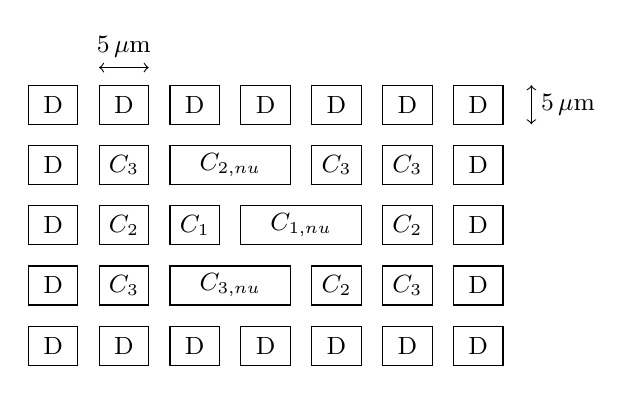
\begin{tikzpicture}[x=.9cm,y=.9cm,font=\small]
\foreach \x in {0,...,6}{
 \draw(\x,0)rectangle++(.7,.55);\node at(\x+.35,.275){D};
 \draw(\x,3.4)rectangle++(.7,.55);\node at(\x+.35,3.675){D};
}
\foreach \y in {.85,1.7,2.55}{
 \draw(0,\y)rectangle++(.7,.55);\node at(.35,\y+.275){D};
 \draw(6,\y)rectangle++(.7,.55);\node at(6.35,\y+.275){D};
}
\foreach \x/\y/\lab in {1/2.55/C_3,4/2.55/C_3,5/2.55/C_3,
1/1.7/C_2,2/1.7/C_1,5/1.7/C_2,1/.85/C_3,4/.85/C_2,5/.85/C_3}{
 \draw(\x,\y)rectangle++(.7,.55);\node at(\x+.35,\y+.275){$\lab$};
}
\draw(2,2.55)rectangle(3.7,3.1);\node at(2.85,2.825){$C_{2,nu}$};
\draw(3,1.7)rectangle(4.7,2.25);\node at(3.85,1.975){$C_{1,nu}$};
\draw(2,.85)rectangle(3.7,1.4);\node at(2.85,1.125){$C_{3,nu}$};
\draw[<->](1,4.2)--node[above]{$5\,\mu\mathrm m$}(1.7,4.2);
\draw[<->](7.1,3.4)--node[right]{$5\,\mu\mathrm m$}(7.1,3.95);
\end{tikzpicture}
\end{center}
The non-unit rectangles have the dimensions tabulated above; the placement sketch is not to scale. Capacitors with the same $C_i$ label are connected in parallel. D denotes a dummy capacitor.

\textbf{Layout Technique \#1 =} Dummies around the entire perimeter.\par
\textbf{Layout Technique \#2 =} Approximately common-centroid placement.
\endgroup
\newpage

\begin{center}
{\sffamily\bfseries\Large Scratch Paper}
\end{center}
\null\vfill
\clearpage
